\documentclass[tikz ,border=30pt]{standalone}
\usepackage{tikz}
\usetikzlibrary{fit,positioning, arrows, intersections}
\usepackage{verbatim}
\usetikzlibrary{fit}

\tikzset{
 plate/.style={draw, shape=rectangle, rounded corners=0.5ex, thick,
    minimum width=3.1cm, text width=3.1cm, align=right, inner sep=10pt, inner ysep=10pt,label={[xshift=-14pt,yshift=14pt]south east:#1}}
}
\begin{document}
\centering
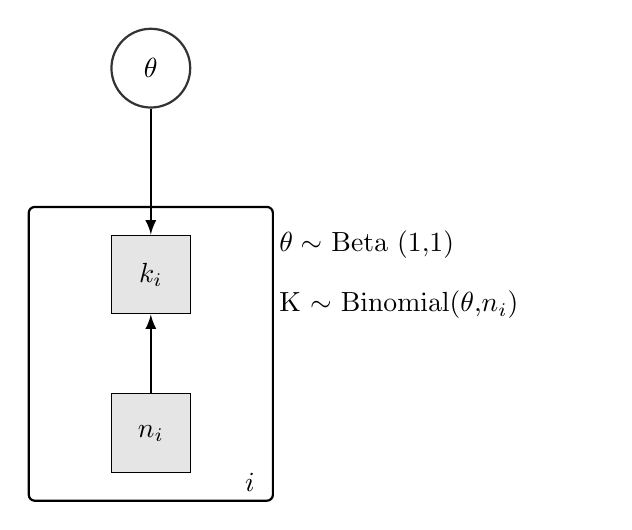
\begin{tikzpicture}
\tikzstyle{circ}=[circle, minimum size = 10mm, thick, draw =black!80, node distance = 16mm]
\tikzstyle{connect}=[-latex, thick]
\tikzstyle{sqr}=[rectangle, draw=black!100, minimum size=10mm]
\baselineskip=32pt
% 2. Nodes
%%%%%%%%%%
\node[sqr, fill=black!10] (K) at (1,0) {$k_i$};
\node[sqr, fill=black!10] (N) [below=of K] {$n_i$};
\node[circ, fill=white!100] (theta) [above=of K] {$\theta$};

\node [text width=4cm] (dists) [right=of K] {
          $\theta \sim $ Beta (1,1)\\[1em]
          K $\sim $ Binomial($\theta$,$n_i$)} ;
\node[plate=$i$, inner sep=10pt, fit=(K) (N)] {};
% 3. Arrows
%%%%%%%%%%%
\path (N)      edge [connect] (K)
      (theta)  edge [connect] (K);

\end{tikzpicture}

\end{document}